\documentclass[crop,border={2pt 2pt 2pt 2pt},tikz]{standalone}
\usepackage{braket}
\usepackage{bbold}
\usepackage{bm}
\usepackage{amsmath}
\usepackage{tikz-3dplot}
% \usepackage{physics}

\usetikzlibrary{backgrounds,decorations.markings, calc}
\tikzset{>=latex}
\tikzset{->-/.style={decoration={
  markings,
  mark=at position .55 with {\arrow{>}}},postaction={decorate}}}
\begin{document}
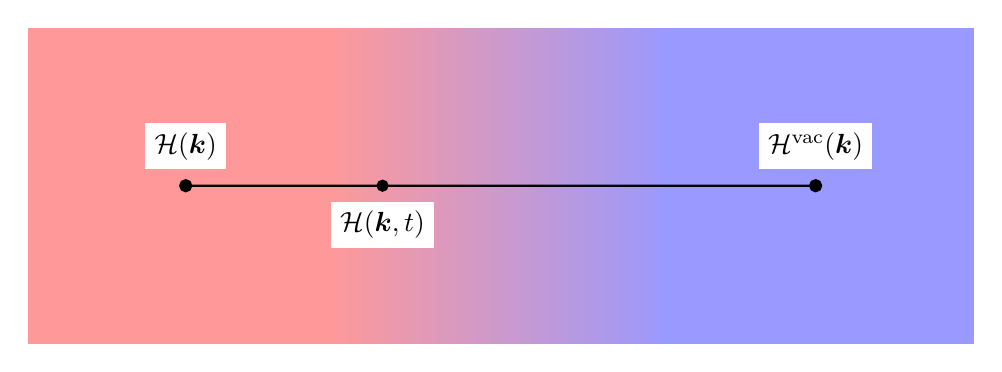
\begin{tikzpicture}[line join = round]
    \draw[fill, red!40!white] (-2,-2) rectangle (2,2);
    \shade[left color = red!40!white, right color = blue!40!white] (1.8,-2) rectangle (6.2,2);
    \draw[fill, blue!40!white] (6,-2) rectangle (10,2);
    \node[fill = white] at (0,0.5) {$\mathcal{H}(\bm k)$};
    \node[fill = white] at (8,0.5) {$\mathcal{H}^{\text{vac}}(\bm k)$};
    \draw[thick, fill] (0,0) circle (2pt) -- (8,0) circle (2pt);
    \draw[fill] (2.5,0) circle (2pt);
    \node[fill = white] at (2.5,-0.5) {$\mathcal{H}(\bm k, t)$};

\end{tikzpicture}
\end{document}